\documentclass{article}
\usepackage[utf8]{inputenc}
\usepackage[german]{babel} % Silbentrennung, Anführungszeichen usw.
%\usepackage[babel,german=quotes]{csquotes}

\usepackage{url}
\usepackage{listings}
\usepackage{color}
\usepackage{graphicx}
\usepackage[a4paper,margin=1in]{geometry}

\usepackage{mathptmx}% http://ctan.org/pkg/mathptmx

\usepackage{array}
\usepackage{multirow}


\definecolor{mygreen}{rgb}{0,0.2,0}
\definecolor{mygray}{rgb}{0.95,0.95,0.95}
\definecolor{mymauve}{rgb}{0.58,0,0.82}

\lstdefinelanguage{mylog}{
  comment=[l]{//},
  morecomment=[s]{/*}{*/}
}

\title{GeoGebra Automatisierte Begründungwerkzeuge\\ \large Ein Tutorial}
\author{Zolt\'an Kov\'acs, Tom\'as Recio und M. Pilar V\'elez\\
Übersetzt von Katharina Schiffler
}

\begin{document}
\lstset{
  basicstyle=\ttfamily,
  columns=fullflexible,
  keepspaces=true,
  breaklines=true,
  backgroundcolor=\color{mygray},
  keywordstyle=\color{blue},
  stringstyle=\color{mymauve},
  ndkeywordstyle=\color{red},
  commentstyle=\color{mymauve},
  identifierstyle=\color{mygreen}
}
%\tolerance10000

\maketitle

\section{Einführung}

Das Softwaretool GeoGebra (\url{http://www.geogebra.org}) ist geeignet zur Unterstützung des Unterrichts der zweidimensionalen euklidischen Geometrie Theorien mit symbolischen Berechnungen. Zu diesem Zweck wurden einige Werkzeuge für den automatischen Beweis und zur Entdeckung von geometrischen Lehrsätzen entwickelt.

Die neuen Technologien im Klassenzimmer befinden sich noch in einer experimentellen Phase. Dieses Dokument fasst die technischen Möglichkeiten zusammen und zeigt auch einige Beispiele.

\section{GeoGebra starten}

GeoGebra ist auf vielen Plattformen verfügbar, wie zum Beispiel
\begin{itemize}
    \item Computer mit verschiedenen Betriebssystemen
    \item Tablets, und
    \item Smartphones.
\end{itemize}
Darüber hinaus sind eingebettete GeoGebra Applets auf Websites verfügbar, speziell auf GeoGebra Materials (\url{https://www.geogebra.org/materials/}) mit Millionen kostenlos verfügbarer Unterrichtsmaterialien.

Die verfügbaren Werkzeuge können unter Umständen variieren. Auch die Benutzererfahrung kann auf den verschiedenen Plattformen unterschiedlich sein: Die symbolischen Berechnungen können ein hohes Ausmaß an Kalkualtionen benötigen und die unterliegenden Hardware- und Softwarekomponenten unterstützen möglicherweise nicht alle Schritte vollständig.

Die vorgeschlagene Plattform für Klassen kann variieren. Die schnellsten Resultate können mit schnellen Computern erzielt werden, aber in diesem Fall muss die Software vom Benutzer heruntergeladen und installiert werden. Manche Beispiele in diesem Tutorial funktionieren unter Umständen nur in der \glqq{}Desktop\grqq{} Version (welche für Microsoft Windows, Apple Macintosh und Linux Computer verfügbar ist). Auf der anderen Seite benötigt die ``Web'' Version keine Installation durch den Benutzer: Diese funktioniert mit einem aktuellen Web Browser und die Lehrerin/der Lehrer kann zum Beispiel eine Liste von Beispielen als GeoGebra Applets für die Klasse unter Verwendung von GeoGebra Materials vorbereiten. Die ``Web'' Version ist allerdings langsamer: Die symbolische Berechnung kann etwas langsamer sein.

GeoGebra funktioniert mittlerweile auch auf Tablets und Smartphones. In manchen Fällen können diese Plattformen schnellere Ergebnisse liefern als die Web Version, aber der kleinere Bildschirm könnte die Benutzer davon abhalten, geometrische Lehrsätze im Detail zu untersuchen. Lehrerinnen und Lehrer sollen bestärkt werden, mit dem Umgang dieser modernen Hilfsmittel zu experimentieren, aber der Einsatz für automatische Beweisführung ist noch nicht erforscht.

An den Werkzeugen zur automatischen Beweisführung wird kontinuierlich gearbeitet. Es ist zu bevorzugen, immer die aktuellste Version zu verwenden. Ein wöchentliches Update kann generell für alle Versionen empfohlen werden, abgesehen vom Mac App Store, welcher ungefähr monatlich aktualisiert wird. Die Liste der neuesten Änderungen kann auf \url{http://dev.geogebra.org/trac/timeline}---eingesehen werden -das ist nur für fortgeschrittene Benutzer und Entwickler. 

\section{Automatische Beweisführung Werkzeuge}

Automatische Beweisführung Werkzeuge sind eine Sammlung von GeoGebra Werkzeugen und Befehlen zur Mutmaßung, Entdeckung, Abstimmung und Beweis geometrischer Axiome in einer dynamischen geometrischen Konstruktion.

Am Anfang muss der Benutzer eine geometrische Figur mit bestimmten Werkzeugen auf dem Hauptfenster in GeoGebra zeichnen. Nach der Konstruktion der Figur kann GeoGebra auf verschiedene Arten die geometrischen Eigenschaften mit verschiedenen Werkzeugen und Einstellungen prüfen:
\begin{enumerate}
    \item Mit \textit{freie Objekte ziehen} ihre abhängigen Objekte können sichtbar erforscht werden.
    \item Das \textit{Beziehung} Werkzeug hilft beim Vergleichen von Objekten und erkennen von Beziehungen.
    \item Mit dem Setzen der  \textit{Spur} eines konstruierten Objektes mit/ohne Bewegung eines Objektes wird sichtbar wenn seine vorhergehenden Objekte geändert werden.
    \item Das \textit{Ortslinie} Werkzeug zeigt die Spur eines Objektes für alle möglichen Posititonen eines vorhergehenden Objektes (wenn es sich auf einem Pfad bewegt).
    \item Mit dem Eintippen von \texttt{Beziehung} oder \texttt{Ortslinie} Befehl in der GeoGebra Befehlszeile können genauere Informationen ausgewählt werden. 
\end{enumerate}
Diese Methoden sind normalerweise bekannt in der GeoGebra community, deshalb sind sie gut dokumentiert und es können einige Beispiele auf GeoGebra Materials (\url{https://www.geogebra.org/materials/}) gefunden werden. Auf der anderen Seite bietet GeoGebra zurzeit auch symbolische automatische Beweisführung Werkzeuge für vermutete geometrische Eigenschaften:
\begin{enumerate}
\setcounter{enumi}{5}
    \item Beziehung Werkzeug und Befehl können zum symbolischen Nachrechnen verwendet werden,
    \item Der \texttt{Ortsliniengleichung} Befehl berechnet das Ergebnis der Ortsliniengleichung mit dem Zeigen der algebraischen Gleichung der graphischen Darstellung genauer.
    \item Der \texttt{Ortsliniengleichung} Befehl kann implicit loci prüfen.
    \item Der \texttt{Einhüllende} Befehl berechnet die Gleichung der Tangente mehrerer Objekte während ein bestimmter Vorgänger sich auf einer Bahn bewegt.
\end{enumerate}

\subsection{Einfache und schwierige Werkzeuge}

GeoGebra liefert die obenstehenden schwierigen Methoden um geometrische Theorien zu unterstützen. Diese Icons sind als schwierige Werkzeuge gedacht, weil sie aufgrund ihrer einfachen Benutzung direkt in der Klasse gezeigt werden können. Es gibt auch andere Wege, um mehr über den mathematischen Hintergrund zu lernen oder einfach zur Fehleranalyse. Diese einfachen Methoden sind im Zusatz aufgelistet und daher nicht empfohlen für den direkten Einsatz mit Schülerinnen und Schülern.

Offensichtlich sind einige der aufgelisteten Methoden einfach und andere schwierige. Bei der Befehlszeile in GeoGebra kann überlegt werden als ein schwierigerer Weg für die meisten Benutzer. Daher kann eine Lehrerin/ein Lehrer zuerst die einfacheren Methoden zeigen und nach einiger Erfahrung der Schülerinnen und Schüler die schwierigeren. 

\subsection{Werkzeuge mit symbolischer Unterstützung}

Wie oben erwähnt liefern einige automatische Beweisführung Werkzeuge symbolische Unterstützung. Dieses Feature erlaubt die Verifizierung einem mathematisch rigorosem Weg allgemeine Aussagen der Elementargeometrie, die vom Benutzer vermutet werden.

Ein allgemeiner Hinweis, dass der Benutzer sollte GeoGebra zur Inbetriebnahme mit``Grafikrechner'' Modus starten. Diese Einstellung zeigt die Bezeichnung auf jedem neu hinzugefügten Objekt. Das kann für Beziehungswerkzeug und -befehl entscheidend sein, wenn die verschiedenen Beziehungen ausgewertet werden. 

In den meisten Fällen sind die Achsen nicht wirklich notwendig: Diese können ausgeschaltet werden, wenn das \textit{Bewegen} Werkzeug aktiv ist. (das ist das linke Icon, das einen Cursor zeigt) mit rechtsklickc in der \textit{Grafik Ansicht} und Auswahl der \textit{Achsen} Einstellung.

In einigen Fälle ist es nicht notwendig, die \textit{Algebra Ansicht} anzuzeigen. Wenn die Gleichungen der impliziten Kurven nicht im Detail betrachtet werden,  kann dies auch durch die Änderung der Bezeichnung erreicht werden, sodass auch der Wert angezeigt wird. (Um das durchzuführen, muss ein Rechtsklick und die Auswahl \textit{Objekt Eigenschaften} durchgeführt werden, der Benutzer muss  \textit{Beschriftung anzeigen} zu \textit{Wert} an dem  \textit{Basis} auswählen.)

GeoGebra Applets können komfortabel genutzt werden, wenn sie auf GeoGebra Materials hochgeladen  sind.
Wenn die Algebra Ansicht verwendet wird, kann es hilfreich sein, die Weite zu vergrößern, bevor das Applet auf GeoGebra Materials hochgeladen wird. Sonst könnte es schwierig für den Benutzer sein, die Befehle einzugeben. Nach dem hochladen in GeoGebra Materials ist es wichtig, die Funktionen des Applets  \textit{Erweiterte Einstellungen},  \textit{Zeige Werkzeugleiste} und \textit{Zeige Befehlszeile} zu überprüfen. Danach sollte eine adäquate Größe für das Applet gewählt werden.


\subsubsection{Das Beziehungswerkzeug und Befehle}

GeoGebras Beziehungswerkzeug und Befehle zeigt ein Fenster, das dem Benutzer Informationen über die Beziehung zwischen zwei oder mehr Objekten gibt.
Dieser Befehl erlaubt dem Benutzer, numerisch herauszufinden, ob (für die gezeichnete Konstruktion mit zugehörigen Koordinaten)
\begin{itemize}
    \item zwei Geraden normal aufeinander stehen,
    \item zwei Geraden parallel sind,
    \item zwei (oder mehr) Objekte (Punkte, Streckenlängen, Polygonflächen) gleich sind,
    \item ein Punkt auf einer Linie oder Kurve liegt,
    \item eine Gerade eine Tangent oder eine Passante einer Kurve ist,
    \item drei Punkte kollinear sind,
    \item drei Geraden übereinstimmend sind (oder parallel),
    \item vier Punkte auf einer Kreisbahn liegen (oder kollinear sind).
\end{itemize}
Manche dieser Überprüfungen können auch symbolisch ausgeführt werden, also der Satz kann generell verifiziert werden (mit beliebigen Koordinaten) und nicht nur für die gezeichnete konkrete Konstruktion.

Mit der Verwendung des Beziehungs \textit{werkzeug} muss der Benutzer auf zwei Objekte klicken um die Mitteilungsbox zu sehen. Alternativ können zwei, drei oder vier Objekte mit dem Auswahlrechteck ausgewählt werden, um die Mitteilungsbox zu erhalten. Um nicht ungewollte Objekte im Applet auszuwählen ist es möglich, diese von der Auswahl auszunehmen, indem man mit einem Rechtsklick und der Auswahl \textit{Objekt Eigenschaften} \textit{Erweitert} auswählt und das Häkchen bei \textit{Auswahl erlaubt}entfernt.

Bei der Verwendung des Beziehungs \textit{befehls} gibt der Benutzer eine der folgenden Formlen in die Befehlszeile ein:
\begin{itemize}
    \item \texttt{Beziehung[ <Objekt>, <Objekt> ]}
    \item \texttt{Beziehung[ \{ <Objekt>, <Objekt> \} ]}
    \item \texttt{Beziehung[ \{ <Objekt>, <Objekt>, <Objekt> \} ]}
    \item \texttt{Beziehung[ \{ <Objekt>, <Objekt>, <Objekt>, <Objekt> \} ]}
\end{itemize}

Wenn die Mitteilungsbox eines oder mehrere zutreffende numerische Aussagen zu dem Objekt zeigt, gibt es unter Umständen eine Schaltfläche  ``Mehr$\ldots$'' , welche die symbolische Unterstützung für die gegebene Aussage zeigt. Bei Klick auf ``Mehr $\ldots$'', wird in Kürze die numerische Aussage zu einer allgemeinen Aussage aktualisiert.

\paragraph{Beispiel (Thaleskreis)}
\begin{center}
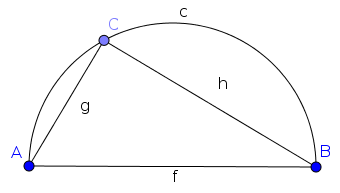
\includegraphics[scale=0.5]{Relation-example}
\end{center}
\begin{enumerate}
    \item Mit dem \textit{Strecke} Werkzeug wird $AB$ konstruiert.
    \item Mit der Auswahl \textit{Halbkreis durch zwei Punkte} Werkzeug wird $c$ erstellt.
    \item Der Punkt $C$ wird auf $c$ erstellt.
    \item Konstruieren Sie die Strecken $AC$ und $BC$ und benennen Sie diese $g$ und $h$.
    \item Vergleichen Sie $g$ und $h$ unter Verwendung des Beziehungswerkzeugs durch Anklicken von $g$ und $h$, oder durch Eintippen von \texttt{Beziehung[g,h]} in der Befehlszeile. Die folgende Mitteilung wird angezeigt:
    \begin{center}
    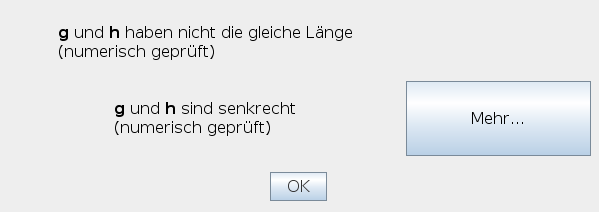
\includegraphics[scale=0.5]{Relation-example-Relation1-de}
    \end{center}
    \item Klicken Sie auf ``Mehr$\ldots$''--- die Mitteilung wird sich wie folgt ändern:
    \begin{center}
    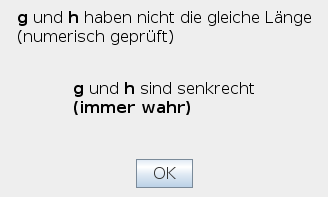
\includegraphics[scale=0.5]{Relation-example-Relation2-de}
    \end{center}
    
\end{enumerate}

Beachten Sie, dass Beziehung (Schritt 5) sucht nach Beziehungen zwischen $g$ und $h$ von den Koordinaten und Gleichungen abhängig von der gezeichneten Konstruktion. Durch Klicken auf ``Mehr$\ldots$'' (Schritt 6) kann verifiziert werden, dass $g$ und $h$ normal aufeinander stehen und für alle Punkte kann $A$ und $B$ kann man Schritt 1 auswählen.

Beziehung zwischen bestimmten Objekten kann unter bestimmten Bedingungen wahr sein, aber nicht zwingend  ``immer''. In diesen Fällen werden genug Voraussetzungen angezeigt. Sonst zeigt GeoGebra nur die Aussage  ``unter bestimmten Voraussetzungen''. Das muss als ``allgemein wahr'' verstanden werden, aber in manchen Einzelfällen (welche eine`minimale Anzahl von Fällen' ist, verglichen mit den allgemeinen Fällen) kann die Aussage falsch sein.

Das symbolische Ergebnis der Beziehung kann auch negativ sein, auch wenn die numerische Überprüfung positiv ist. Zum Beispiel, wenn man zwei Punkte $P=(0,0)$und $Q=(0,0)$ definiert, kann die Beziehung diese numerisch vergleichen, aber das symbolische Ergebnis kann ergeben, dass``$P$ und $Q$ gleich sind (aber nicht allgemein wahr)''.

Eine komplette Übersicht der verschiedenen Ergebnisse der Beziehung könnene im Anhang gefunden werden. \ref{Erklaerungstabelle} auf der Seite \pageref{Erklaerungstabelle}.

\subsubsection{Die Ortsliniengleichung \texttt{Ortsliniengleichung} Befehl}

Dieser Befehl berechnet die Gleichung einer Ortslinie und zeichnet diese als implizite Kurve. Es gibt zwei Möglichkeiten der Nutzung:

\begin{itemize}
\item\textbf{Explizite Ortslinie.}
Gegeben ist ein Anfangspunkt $\cal{I}$ auf einer Strecke $\cal{P}$, einige Konstruktionsschritte und ein Endpunkt $\cal O$. Die Aufgabe ist, die Gleichung von $\cal E$ of $\cal O$ zu bestimmen, wenn sich  $\cal I$ auf $\cal P$ bewegt, und dann  $\cal E$ zu bestimmen. $\cal I$ ist für gewöhnlich \textit{beweger} genannt, $\cal O$ ist die \textit{Spur}. $\cal E$ heißt \textit{Ortsliniengleichung} und ihre grafische Visualisierung ist die \textit{Ortslinie}.

Die Schreibweise des Befehls ist:
\begin{center}
    \texttt{Ortsliniengleichung[ <Punkt Spur>, <Punkt Beweger> ]}.
\end{center}

\paragraph{Beispiel}
\begin{center}
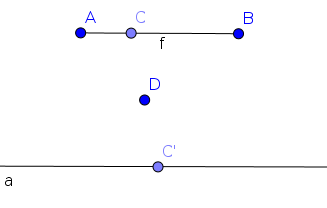
\includegraphics[scale=0.5]{LocusEquation-example-explicit}
\end{center}
\begin{enumerate}
    \item Unter Verwendung des \textit{Strecke} Werkzeug wird $AB$ konstruiert. Es wird eine automatische Strecke $f$ konstruiert.
    \item Setzen Sie Punkt $C$ auf $f$.
    \item Erstellen Sie Punkt $D$ mit dem \textit{Punkt} Werkzeug.
    \item Mit dem \textit{über Punkt spiegeln} Werkzeug spiegeln Sie $C$ über $D$. Damit erstellen Sie Punkt $C'$.
    \item Geben Sie \texttt{Ortsliniengleichung[C',C]} in die Befehlszeile ein. Nun wird die implizite Kurve $a$ berechnet und gezeichnet. Das sollte eine Strecke (das Spiegelbild von $f$ über $D$ sein), aber GeoGebra zeichnete $f$ als Gerade statt einer Strecke (aus algebraischen geometrischen Gründen), da das Spiegelbild ebenfalls eine Gerade ist.
    \item Versuchen Sie, die verschiebbaren Objekte zu ziehen. Es kann gezeigt werden, dass das Spiegelbild einer Strecke über einen Punkt immer parallel zum Urbild ist.
\end{enumerate}

\item \textbf{Implizite Ortslinie.}
Gegeben ist ein Anfangspunkt $\cal I$, entweder als beliebiger Punkt oder auf einer Strecke $\cal P$. Es sind auch einige Konstruktionsschritte gegeben. Der Benutzer behauptet eine Boolsche Bedingung $\cal C$ auf einige Objekte der Konstruktion. Die Aufgabe ist, eine Gleichung $\cal E$ für alle Punkte $\cal{I}'$ aufzustellen, sodass $\cal{I}=\cal{I}'$,  $\cal{C}$ erfüllt. Wieder heißt  $\cal{E}$ Ortsliniengleichung und ihre grafische Interpretation ist die Ortslinie.

Die Schreibweise des Befehls ist:
\begin{center}
    \texttt{Ortsliniengleichung[ <Boolscher Ausdruck>, <Punkt> ]}.
\end{center}

%\vfill\eject %% no idea how to do it elegantly

\paragraph{Beispiel}
\begin{center}
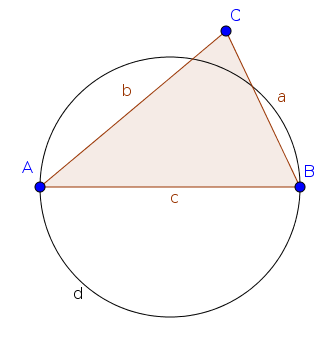
\includegraphics[scale=0.5]{LocusEquation-example-implicit}
\end{center}
\begin{enumerate}
    \item Mit dem \textit{Polygon} Werkzeug wird ein Dreieck $ABC$ konstruiert.Die Strecken $a$, $b$ und $c$ werden automatisch von GeoGebra erstellt.
    \item Es wird \texttt{Ortsliniengleichung a\^{}2+b\^{}2==c\^{}2,C]} in der Werkzeugleiste eingegeben. Jetzt wird die implizite Kurve $d$ berechnet und gezeichnet, welche wie ein Kreis aussieht.
    Bedenken Sie, dass \textit{zwei} gleiche Zeichen eingegeben werden müssen; eine andere Möglichkeit ist, $\stackrel{?}{=}$ zu verwenden. (durch anklicken von \framebox{$\alpha$} Icon, oder durch Einfügen des Symbols von einer externen Applikation mit Copy and Paste).
    \item Versuchen Sie nun, die beweglichen Objekte zu ziehen. Es kann gezeigt werden, dass wenn $C$ auf einem Kreis liegt, dessen Durchmesser auf $AB$ liegt, wegen der rechtwinkeligen Eigenschaft des Dreiecks---$a^2+b^2=c^2$ gilt.
\end{enumerate}

\end{itemize}

Eine Boolsche Bedingung kann sein:
\begin{itemize}
\item Eine Gleichung mit der Bezeichnung der Strecken, e.g.~\texttt{a\^{}2+b\^{}2==c\^{}2}.
\item Eine Gleichheit von zwei Geometrischen Objekten, e.g.~\texttt{A==B}. Beachten Sie, dass \textit{zwei} gleiche Zeicehn eingegeben werden müssen; es gibt auch andere Möglichkeiten
\begin{itemize}
    \item $\stackrel{?}{=}$ (durch Anklicken des \framebox{$\alpha$} Icon, oder durch Einfügen des Symbols von einer externen Applikation mit Copy and Paste.
    \item Alternativ, \texttt{SindGleichl[A,B]} für die gesamte Boolsche Bedingung.
\end{itemize}
\item Eine Überprüfung, ob zwei geometrische Objekte kongruent sind, e.g.~\texttt{SindKongruent[c,d]}.
\item Eine Überpüfung, ob ein Punkt auf einer Strecke, einer Gerade oder einem Kreis liegt, e.g.~\texttt{A$\in$c}.
\item Eine Überprüfung, ob zwei Geraden oder Strecken parallel sind, e.g.~\texttt{p$\parallel$q}. Hier kann auch \texttt{SindParallel[p,q]} verwendet werden.
\item Eine Überprüfung, ob zwei Geraden oder Strecken normal aufeinander stehen, e.g.~\texttt{p$\perp$q}. Hier kann auch \texttt{ArePerpendicular[p,q]} verwendet werden.
\item \texttt{SindKollinear[A,B,C]} prüft, ob die Punkte $A$, $B$ und $C$ kollinear sind.
\item \texttt{SindKongruent[d,e,f]} prüft, ob die Geraden $d$, $e$ und $f$ kongruent sind.
\item \texttt{SindKonzentrisch[A,B,C,D]} prüft, ob die Punkte $A$, $B$, $C$ und $D$ konzentrisch sind.
\end{itemize}

\subsubsection{Der \texttt{Einhüllende} Befehl}

Dieser Befehl berechnet die Gleichung einer Tangente zu einer Gruppe von Objekten mit einem bestimmten Vorgänger auf einer Strecke.

Präziser gesagt, ist ein Anfangspunkt $\cal{I}$ auf einer Strecke $\cal{P}$,einige Konstruktionsschritte und ein Endpunkt $\cal O$ gegeben, entweder eine Gerade oder ein Kreis. Die Aufgabe besteht darin, die Gleichung $\cal E$ einer Kurve $\cal C$, welche die Tangente zu $\cal O$ ist, aufzustellen, wenn sich $\cal I$ auf $\cal P$. Am Ende ergibt sich $\cal E$. $\cal I$ wird der Beweger genannt. $\cal E$ wird die \textit{Einhüllende Gleichung} genannt, und ihre graphische Darstellung ist die \textit{Einhüllende}.

%\vfill\eject %% no idea how to do it elegantly

\paragraph{Beispiel}
\begin{center}
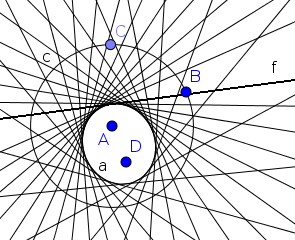
\includegraphics[scale=0.5]{Envelope-example}
\end{center}
\begin{enumerate}
    \item Mit dem \textit{Kreis mit Mittelpunkt durch Punkt} Werkzeug, wird ein Kreis $c$ mit dem Mittelpunkt $A$und dem Umkreispunkt $B$ konstruiert.
    \item Setzen Sie Punkt $C$ auf $c$.
    \item Erstellen Sie einen beliebigen Punkt $D$ in $c$.
    \item Konstruieren Sie die \textit{Mittelsenkrechte} $f$ der Strecke $CD$ unter Verwendung der Endpunkte.
    \item Geben Sie \texttt{Einhüllende[f,C]}in der Befehlszeile ein. Die implizite Kurve $a$ wird berechnet und gezeichnet. Diese sieht aus wie eine Ellipse.
\end{enumerate}


\subsection{Technische Notizen}

Die folgenden Notizen sind wichtige Einschränkungen für jedes Automatische Begründungswerkzeug in GeoGebra, symbolische Berechnungen nutzt:
\begin{itemize}
\item Es werden nicht alle GeoGebra Werkzeuge und Konstruktionsschritte unterstützt.
\item Die unterstützten Werkzeuge funktionieren nur für eine beschränkte Menge an geometrischen Objekten, zum Beispiel die Verwendung von Punkten, Geraden, Kreisen, Kegel.
\item Abschnitte von Strahlen und Geraden werden als unendliche Geraden behandelt. Kreisbögen werden wie Kreise behandelt.
\item Zu komplizierte Ortslinien- oder Einhüllende-Berechnungen können in der Algebra Ansicht als "undefiniert" dargestellt werden.
\item Beziehungs-Beweise, deren Inhalt zu kompliziert ist, werden die Mitteilung "möglicherweise allgemein wahr" anzeigen. Die Interpretation dafür ist, dass es GeoGebra nicht möglich ist, zu entscheiden, ob die Beziehung im allgemeinen wahr ist, aber die numerischen Ergebnisse lassen darauf schließen.
Das heißt, die Beziehung kann auch im allgemeinen falsch sein.
\item Wenn es keine Ortslinie oder Einhüllende gibt, ist die implizite Kurve die leere Menge $0=1$. Zum Beispiel: Für einen beliebigen Punkt $P$
\begin{center}
\texttt{Ortsliniengleichung[false,P]}
\end{center}
zeigt die leere Menge.
\item Wennn die Ortslinie oder die Einhüllende die ganze Ebene ist, hat die implizite Kurve die Gleichung $0=0$. Zum Beispiel: Für einen beliebigen Punkt $P$
\begin{center}
\texttt{Ortsliniengleichung[true,P]}
\end{center}
zeigt die ganze Ebene.
\item Manchmal werden zusätzliche Verzweigungen erscheinen, die nicht in der ursprünglichen Ortslinie oder Einhüllenden waren.
\item Der Graph der impliziten Kurve kann in manchen Fällen ungenau sein.
\end{itemize}

\section{Verwendung in der Klasse: Vermutung, Beweis und Verallgemeinerung}

Technisch gesehen ist das Beziehungswerkzeug das einfachsten symbolische Werkzeug aus der obigen Liste. Auf der anderen Seite können manche Unterrichtssituationen den Einsatz andere Werkzeuge, oder den Einsatz mehr als eines Werkzeuges erfordern, möglicherweise auch in einer anderen Reihung als in der obigen Liste.

\subsection{Satz des Thales}

In vielen traditionellen Mathematikstunden wird der Satz des Thales in einer expliziten Form unterrichtet: Wenn $C$ auf einem Halbkreis liegt, sind die Strecken $g$ und $h$ normal aufeinander. Tatsächlich kann dieser Lehrsatz mit einer offenen Frage formuliert werden: \textit{Sei $ABC$ ein beliebiges Dreieck. Was ist die geometrische Ortslinie von $C$, wenn der Winkel bei $C$ ein rechter Winkel sein soll?}

Bei diesem Zugang kann es sinnvoller sein, den technisch anspruchsvolleren \texttt{Ortsliniengleichung[g$\perp$h,C]} Befehl zuerst zu verwenden und dann die Konstruktion mit dem Beziehungswerkzeug oder -befehl zu vollenden. Der Output des   \texttt{Ortsliniengleichung} Befehl kann den Schülerinnen und Schülern zeigen, dass die Kurve ein Kreis ist. Die Algebra Ansicht zeigt die Gleichung der Kurve, das könnte unter Umständen für jüngere Schülerinnen und Schüler verwirrend sein.

Schließlich kann der Satz des Thales durch das eingeschriebene Dreieck in einen Halbkreis verallgemeinert werden. In diesem Fall ist die Bedingung nicht mehr $g\perp h$, sondern der Winkel der beiden veränderlichen Strecken zu einer fixen. GeoGebra unterstützt diese Art der Erhebung mit der Schreibweise.
\begin{center}
\texttt{Ortsliniengleichung[SindKongruent[$\alpha$,$\beta$],C]}
\end{center}
wenn $\alpha$ fix ist und $\beta=\angle{ACB}$.

Zusammenfassend, bei diesem Zugang
\begin{enumerate}
    \item wird eine implizite Ortslinie mit GeoGebra berechnet,
    \item wird von den Schülerinnen und Schülern eine Vermutung aufgestellt, wie die Kurve aussieht,
    \item wird die Vermutung mit dem Beziehungswerkzeug oder -befehl in GeoGebra überprüft,
    \item kann der Beweis von den Schülerinnen und Schülern optional handschriftlich durchgeführt werden,
    \item wird der Satz des Thales mit den impliziten Ortslinien in GeoGebra verallgemeinert -- als zukünftiges Experiment für die Schülerinnen und Schüler.
\end{enumerate}

\subsection{Weitere Beispiele}

Die Dreiecksungleichung kann in eine Gleichung übersetzt werden, die in eine Erforschung der degenerierten Dreiecke geändert werden kann. Als Verallgemeinerung kann die künstliche Definition von konischen Segmenten erwähnt werden.

Eine andere Anwendung ist eine Verzweigung der Ortsliniengleichung im Dreieck $ABC$ mit der Bedingung $a\stackrel{?}{=}b$, dazu muss $C$ gefunden werden (Schritt 1). Natürlich muss $C$ auf der Streckensymmetrale  $AB$ liegen (Schritt 2). Dass  $C$ explizit auf der Streckensymmetrale liegt, bestätigt GeoGebra, als $AC=BC$ , wenn man die Berechnung mit dem Beziehungswerkzeug startet (Schritt 3). Nach dem Beweis des Satzes mit traditionellen Methoden (Schritt 4) kann eine Verallgemeinerung durch das Eintippen des Befehles\texttt{Ortsliniengleichung[a==2b,C]}: erhalten werden. Dies kann auch ein interessantes Experiment für fortgeschrittene Schülerinnen und Schüler sein (Schritt 5).

\subsection{Ein ausgearbeitetes Beispiel: Der Satz von der Mittelparallelen im Dreieck}

Diese Schritt für Schritt Anleitungen sind ein möglicher Weg, den Satz von der Mittelparallelen im Dreieck mit den automatischen Beweiswerkzeugen in GeoGebra durchzuführen.

\paragraph{Schritt 1}
\begin{center}
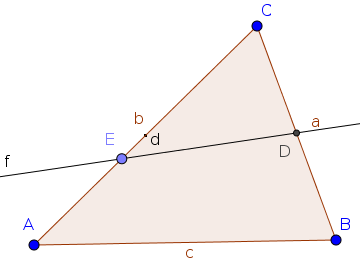
\includegraphics[scale=0.5]{classroom1}
\end{center}
\begin{enumerate}
    \item Mit Verwendung des \textit{Polygon} Werkzeuges wird ein Dreieck $ABC$ konstruiert. Dabei werden automatisch die Strecken $a$, $b$ und $c$ konstruiert.
    \item Mit Verwendung des \textit{Mittelpunkt} Werkzeuges, wird der Mittelpunkt $D$ von $a$ konstruiert..
    \item Erstellen Sie Punkt $E$ auf $b$.
    \item Erstellen Sie die Gerade $f$, die $D$ und $E$ verbindet.
    \item Fragen Sie GeoGebra, wie $E$ sein muss, damit $f$ parallel zu $c$ ist: Tippen Sie\texttt{Ortsliniengleichung[c$\parallel$f,E]} in die Eingabezeile. Dadurch wird die implizite Kurve $d$ berechnet und konstruiert. Diese scheint ein einziger Punkt zu sein. Achtung: Es könnte hilfreich sein, die Linienstärke der impliziten Kurve $d$ zu ändern und auch die Schriftgröße zu ändern, damit diese nicht von anderen Objekten versteckt wird. Beide Einstellungen können im Fenster Grundeinstellungen geändert werden.
\end{enumerate}
\paragraph{Schritt 2}
\begin{center}
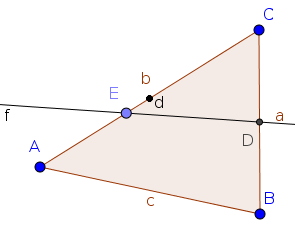
\includegraphics[scale=0.5]{classroom2}
\end{center}
\begin{enumerate}
    \item[6.] Ziehen Sie an den beweglichen Objekten und zeigen Sie, dass $E$ der Mittelpunkt von $b$ sein muss.
    \item[7.] Um diese Vermutung zu bestätigen, erstellen Sie den Mittelpunkt $F$ der Strecke $b$ (und passen Sie die Beschriftung von $d$ und $F$, um Überschneidungen zu vermeiden.). Ziehen Sie erneut an den beweglichen Objekten.
\end{enumerate}
\paragraph{Schritt 3}
\begin{center}
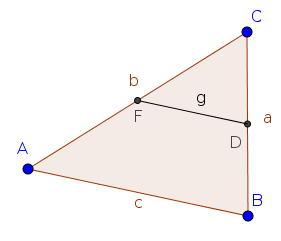
\includegraphics[scale=0.5]{classroom3}
\end{center}
\begin{enumerate}
    \item[8.] Machen Sie die Objekte $E$, $f$ und $d$ unsichtbar, indem Sie diese verstecken.
    \item[9.] Verbinden Sie $D$ und $F$ mit einer Strecke $g$.
    \item[10.] Verwenden Sie das  \textit{Beziehung} Werkzeug, um $c$ und $g$ zu vergleichen. Sie sind parallel.
    \item[11.] Klicken Sie auf ``Mehr $\ldots$'' im Pop Up Fenster und überprüfen Sie symbolisch, dass sie parallel sind.
\end{enumerate}
\begin{center}
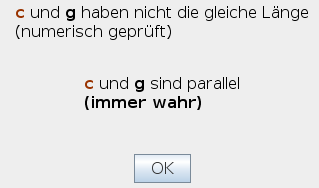
\includegraphics[scale=0.5]{classroom3-Relation-de}
\end{center}
Die Schülerinnen und  Schüler machen mit Schritt 4 weiter, wenn sie einen eleganten Weg benötigen, diese Behauptung zu beweisen, oder hören an dieser Stelle auf, wenn keine weitere Zeit in der Klasse für dieses Problem aufgewendet werden soll.

Auch in Schritt 5 können weitere Fragen auftreten. $c$ und $g$ haben nicht die selbe Länge, können aber unter Verwendung der Länge von $c$ berechnet werden? Vielleicht $c=1.5\cdot g$, oder vielleicht mehr? Der GeoGebra Befehl \texttt{Relation[c,1.5g]} ergibt, dass $c$ und $1.5g$ nicht gleich sind, aber es vielleicht eine andere Konstante als $1.5$ gibt, die eine positive Antwort erzeugt. $\ldots$ Auch wenn keine Zeit für weitere Arbeiten in der Klasse bleibt, werden manche Schülerinnen und Schüler diese Fragen interessant finden und alleine oder in Gruppen darüber nachdenken, sinnvollerweise  \textit{independently}, unter Verwendung des Computers als Experten.

\section{Beschränkung: Eine Fallstudie des Satzes von Thales}

Intuitive Benutzung des GeoGebra automatischen Beweiswerkzeuges kann unter Umständen unerwartete Ergebnisse hervorbringen. Diese Unterteilung erklärt einige häufige Fehler bei der Benutzung.

Unterschiedliche Zugänge bei der Erstellung des Satzes von Thales werden diskutiert.

\paragraph{Zugang 1}
\begin{center}
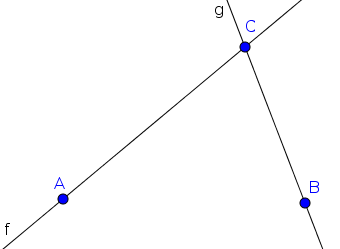
\includegraphics[scale=0.5]{limitations-Thales1-1}
\end{center}
\begin{enumerate}
    \item Erstellen Sie die Punkte $A$, $B$ und $C$.
    \item Erstellen Sie die Geraden $f=AC$, $g=BC$.
    \item Überprüfen Sie das Ergebnis des Befehls \texttt{Beziehung[f,g]}: ``$f$ schneidet $g$''.
    \item Fragen Sie GeoGebra über geometrische Voraussetzungen von $f\perp g$:
\begin{center}\texttt{Ortsliniengleichung[f$\perp$g,C]}.\end{center}
Eine implizite Kurve $a$ , die kreisförmig aussieht, wird gezeigt.
    \item Bewegen Sie $C$ so nahe wie möglich an die implizite Kurve. Nun wird \texttt{Relation[f,g]} noch immer aussagen, dass ``$f$ schneidet $g$''. \textbf{Warum? Weil der Punkt $C$ nicht direkt auf der Kreisbahn liegt. Wir müssen den Punkt exakt auf di Kreisbahn legen.}
    \begin{enumerate}
      \item Versuchen Sie, den Punkt $C$ direkt auf die implizite Kurve $a$ zu setzen. Verwenden Sie dazu das  \textit{Attach / Detach Point} Werkzeug. \textbf{GeoGebra erlaubt das nicht, weil per Definition $a$ auf $C$ liegt, und das würde keinen Sinn ergeben.}
      \item Erstellen Sie stattdessen einen neuen Punkt $D$, den Sie direkt auf die implizite Kurve setzen. Das erlaubt GeoGebra. Erstellen Sie auch die Geraden $h=AD$, $i=BD$.
\begin{center}
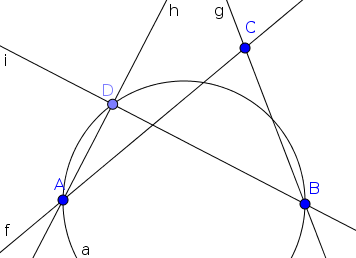
\includegraphics[scale=0.5]{limitations-Thales1-2}
\end{center}
      \item Überprüfen Sie das Ergebnis des Befehls \texttt{Beziehung[h,i]}: ``$h$ und $i$ sind normal aufeinander'' mit einer numerischen Überprüfung. Durch Klicken auf ``Mehr$\ldots$''ist das Ergebnis ``vielleicht immer richtig''. \textbf{Warum? Weil GeoGebra die darunterliegenden implizite Kurve als das Ergebnis einer teilweisen Konfiguration der Konstruktion interpretiert. Mit anderen Worten: eine implizite Kurve ist ein numerisches Objekt, sie hat keine symbolische Bedeutung. Daher sind symbolische Überprüfungen basierend auf einer impliziten Kurve nicht möglich. Hier ist GeoGebra nur optimistisch, was die Wahrheit der Vermutung betrifft, aber die Software ist nicht fähig, dies zu prüfen.}
      \item Der eigentliche Weg, die Schritte in dieser Vermutung zu einem Ende zu führen ist,  einen Kreis mit dem Durchmesser $AB$ mit dem Kreiswerkzeug zu konstruieren, zum Beispiel mit dem \textit{Halbkreis durch 2 Punkte} Werkzeug, nachdem $D$ von $a$ abgetrennt wurd und dann $a$ unsichtbar zu machen. Dann kann $D$ zu dem Halbkreis hinzugefügt werden.
\begin{center}
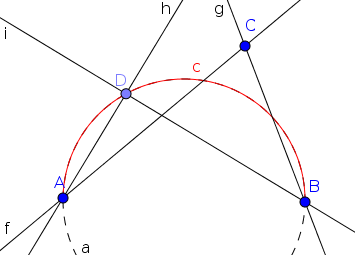
\includegraphics[scale=0.5]{limitations-Thales1-3}
\end{center}
      (Optional kann die implizite Kurve auch durch eine andere Formatierung sichtbar gemacht werden. In diesem Beispiel wurde eine andere Formatierung auch für den Halbkreis verwendet. Zum Schluss zeigt \texttt{Beziehung [h,i]} positive Ergebnisse, sowohl numerisch, als auch symbolisch.
    \end{enumerate}
\end{enumerate}


\paragraph{Zugang 2}
\begin{center}
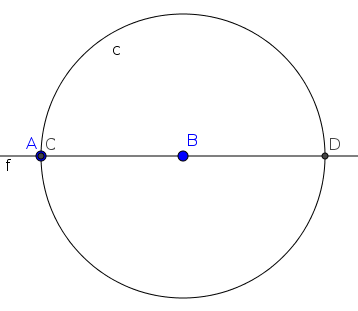
\includegraphics[scale=0.5]{limitations-Thales2-1}
\end{center}
\begin{enumerate}
    \item Erstellen Sie die Punkte $A$ und $B$.
    \item Erstellen Sie den Kreise $c$ mit dem Mittelpunkt $B$ durch $A$.
    \item Konstruieren Sie die Gerade $f$ durch Verbinden der Punkte $A$ und $B$.
    \item Erstellen Sie die Schnitpunkte $C$ und $D$ von $c$ und $f$. (Vielleicht müssen sie die Beschriftung von $A$ verschieben, um Überschneidungen mit der Beschriftung von $C$ zu vermeiden.)
    \item Erstellen Sie Punkt $E$ auf $c$.
    \item Konstruieren Sie die Geraden $g=AE$, $h=DE$.
\begin{center}
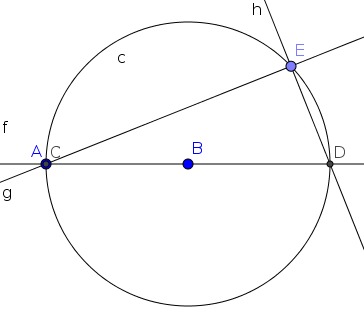
\includegraphics[scale=0.5]{limitations-Thales2-2}
\end{center}
    \item Vergleichen Sie $g$ und $h$ unter Verwendung von \texttt{Beziehung[f,g]}. Das numerische Ergebnis ist richtig, aber GeoGebra sagt, dass die Orthogonalität von $f$ und $g$ nicht grundsätzlich richtig ist. \textbf{Warum? Als $C$ und $D$ konstruiert wurden, wurde nicht definiert, welche welche ist. Daher ist die sichtbare Voraussetzung, dass $A=C$ falsch ist---die andere Möglichkeit $A=D$ muss auch als mögliche Voraussetzung erlaubt sein. In diesem anderen Fall sind $f$ und $g$ natürlich nicht normal aufeinander, sondern identisch.}
\begin{enumerate}
      \item Stattdessen wird die Definition von $g$ zu $g=CE$ geändert. Jetzt wird die Beziehung zwischen $g$ und $h$ richtig gewertet, auch im symbolischen Fall.
      \item Eine andere Möglichkeit ist, nicht beide Schnittpunkte $C$ und $D$ zu konstruieren, sondern nur einen der beiden (Unterschieder zu $A$). Das ist möglich, indem man in die Nähe der Schnittpunkte des Diagramms klickt.
\begin{center}
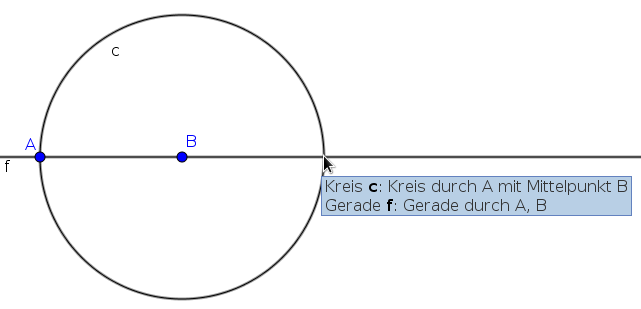
\includegraphics[scale=0.5]{limitations-Thales2-3-de}
\end{center}
      Jetzt wird mit der Konstruktion von  $D$ (durch erstellen auf $c$), $g=AD$ und $h=CD$, weitergemacht.\texttt{Beziehung[f,g]} wird das richtige Ergebnis numerisch und symbolisch zeigen.
\begin{center}
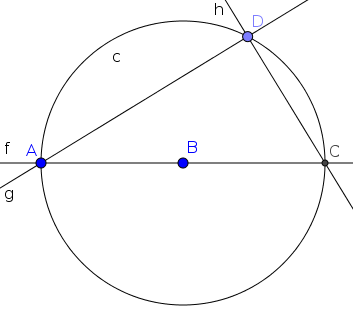
\includegraphics[scale=0.5]{limitations-Thales2-4}
\end{center}
      \textbf{Warum? In diesem Diagramm zeigt GeoGebra, dass sich $C$ von $A$ grundsätzlich unterscheidt. (der Spezialfall $A=C$ wird ausgeschlossen von dem symbolisichen Beweis zur Orthogonalität, aber sogar in diesesm Spezialfall wäre die Behauptung der Orthogonalität wahr, das symbolische Ergebnis ist "immer wahr").}
    \end{enumerate}
\end{enumerate}


\section{Anhang}
\subsection{Einfache GeoGebra Werkzeuge}

Automatische Beweisführungswerkzeuge in GeoGebra werden abgerundet durch einige einfach Werkzeuge, die zum zusätzlichen Lernen über exaktere geometrische Eigenschaften.

\subsubsection{Der \texttt{Beweis} Befehl}
Der \texttt{Beweis} Befehl entscheidet, ob eine geometrische Aussage im allgemeinen wahr ist. Es hat drei mögliche Ergebnisse:
\begin{itemize}
    \item \textit{wahr} bedeutet, dass die Aussage immer wahr ist, oder wahr unter einigen degenerierten Bedingungen.
    \item \textit{falsch} bedeutet, dass die Aussage im allgemeinen falsch ist. GeoGebra nutzt algebraische Geometrie in manchen Fällen, um solche Fragen zu entscheiden. In algebraischer Geometrie ``allgemein wahr'' (wahr in `den meisten'' Fällen) und ``im Allgemeinen falsch'' (falsch in ``den meisten'' Fällen) sind nicht gegenseitige Eigenschaften, sondern, eine Aussage kann nicht ``im Allgemeinen wahr'' und nicht ``im Allgemeinen falsch'' zur selben Zeit sein. GeoGebra interpretiert diesen speziellen Fall als\textit{falsch} (wenn es nicht im Allgemeinen wahr ist).
    \item \textit{nicht definiert} bedeutet, dass GeoGebra aufgrund verschiedener Ursachen keine Entscheidung treffen kann:
    \begin{itemize}
        \item Die Aussage kann nicht in ein Modell übersetzt werden, das erforscht werden kann. Das bedeutet normalerweise, dass die Algebraisierung der Aussage nicht durchgeführt werden kann, aufgrund
        \begin{itemize}
            \item theoretischer Unmöglichkeit (e.g.~ Verwendung einer transzendenten Funktion als Konstruktionsschritt, z.B Sinus von $x$),
            \item fehlende Implementation in GeoGebra.
        \end{itemize}
        \item Die übersetzte Aussage in algebraischer Geometrie ist zu schwierig zu lösen. Das kann einerseits bedeuten, dass es zu viele Variablen gibt, oder die Gleichungen sind mit einem Algorithmus schwierig zu bearbeiten. Das führt entweder zu einem Timeout oder der Platz im Hauptspeicher reicht nicht aus.
        \item Der Lösungsalgorithmus konnte die Situation prüfen, aber das Ergebnis ist nicht eindeutig: entweder ist die Behauptung falsch, oder sie ist wahr unter bestimmten Bedingungen. Aber der Algorithmus konnte nicht feststellen, welcher Fall vorliegt.
        \item Es gab eine interne Störung in GeoGebra während der Berechnungen.
    \end{itemize}
\end{itemize}

% Prevent putting the image on the next page.
% \vfill\eject % FIXME
% not needed in German

\paragraph{Beispiel}
\begin{center}
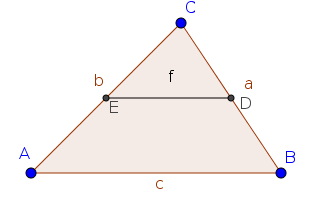
\includegraphics[scale=0.5]{Prove-example}
\end{center}
\begin{enumerate}
\item Konstruieren Sie das Dreieck $ABC$ mit dem \textit{Vieleck} Werkzeug.
\item Konstruieren Sie die Mittelpunkte $D$ und $E$ der Seiten $a$ und $b$,mit dem \textit{Mittelpunkt} Werkzeug.
\item Unter Verwendung des \textit{Strecke} Werkzeug, konstruieren Sie $f$ durch Verbinden mit $D$ und $E$.
\item Geben Sie \texttt{Beweis[f$\parallel$c]} ein, um zu zeigen, dass \textit{wahr} in der Algebra Ansicht als Boolscher Wert $d$ angezeigt wird. Achten Sie darauf, dass das Parallel Zeichen eingegeben werden muss, entweder durch:
\begin{itemize}
\item die Liste der mathematischen Symbole durch Klicken auf das \framebox{$\alpha$} Icon in der Eingabezeile, oder
\item externe Eingabe des Symbols mit Copy and Paste.
\item Alternativ kann \texttt{f$\parallel$c} auch durch \texttt{AreParallel[f,c]} ersetzt werden.
\end{itemize}

\item Geben Sie \texttt{Beweis[c==3f]} ein. Jetzt ist die Antwort \textit{undefiniert}, weil GeoGebra nicht entscheiden kann, ob die Aussage falsch oder wahr ist unter bestimmten Bedingungen. In diesen Fällen kann der Befehl \texttt{PrüfeDetails} helfen. (siehe unten). Beachten Sie, dass \textit{zwei} gleiche Zeichen eingegeben werden müssen; andere Möglichkeiten der Verwendung sind:
\begin{itemize}
    \item \texttt{Prüfe[c$\stackrel{?}{=}$3f]}, oder
    \item \texttt{Prüfe[AreEqual[c,3f]]}.
\end{itemize}

\end{enumerate}

\subsubsection{The \texttt{PrüfeDetails} Befehl}
Der \texttt{PrüfeDetails} Befehl hat ähnliches Verhalten wie der \texttt{Beweis}Befehl, aber es kann verschiedene Algorithmen im Entscheidungsprozess verwenden und und könnte mehr Informationen des Ergebnisses zeigen. Es gibt drei mögliche Ergebnisse:
\begin{itemize}
    \item \textit{\{true\}} bedeutet, dass die Aussage immer wahr ist.
    \item \textit{\{true, \{$\ldots$\}\}} wenn die Aussage unter bestimmten, nicht-degenerierten oder essentiellen Bedingungen wahr ist: Diese Bedingungen sind in Klammern geschrieben. (Wenn die Liste bleibt, bedeutet das, dass keine künstliche Übersetzung gefunden werden konnte ``$\ldots$''.) Wenn die Verbindung der Verneinten Bedingungen wahr ist, dann ist die Aussage wahr.
    \item \textit{\{false\}} bedeutet, dass die Aussage im Allgemeinen falsch ist. Die Kommentare dazu finden Sie beim \texttt{Beweis} Befehl, falls Sie weitere Details benötigen.
\end{itemize}
\paragraph{Beispiel (fortgesetzt)}
\begin{enumerate}
\setcounter{enumi}{5}
    \item Geben Sie \texttt{PrüfeDetails[c==3f]} ein. Jetzt ist die Antwort \textit{\{false\}}.
    \item Geben Sie \texttt{PrüfeDetails[c==2f]} ein. Jetzt ist die Antwort \textit{\{true\}}.
\begin{center}
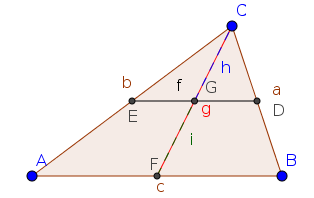
\includegraphics[scale=0.5]{ProveDetails-example-1}
\end{center}
    \item Sei $F$ der Mittelpunkt von $c$,und die Strecke $CF$ wird in $g$ umbenannt. Sei $G$ der Schnittpunkt von $f$ und $g$. Zum Schluss werden noch die Strecken $CG$ und $FG$ in $h$und $i$ umbenannt. In diesem Falle wird \texttt{PrüfeDetails[h==i]} wieder \textit{\{true,\{``AreCollinear[A,B,C]''\}\}}, was bedeutet, dass, wenn $A$, $B$ und $C$ nicht kollinear sind, ist $h=i$.
\end{enumerate}

\paragraph{Ein weiteres Beispiel}
\begin{center}
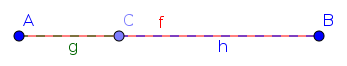
\includegraphics[scale=0.5]{ProveDetails-example-2}
\end{center}
\begin{enumerate}
    \item Sei $AB$ eine Strecke, umbenannt in $f$.
    \item Sei $C$ ein Punkt auf $f$.
    \item Die Strecken $AC$ und $BC$ werden in  $g$ und $h$ umbenannt.
    \item Geben Sie \texttt{PrüfeDetails[f==g+h]} ein. Jetzt ist die Antwort
    \begin{center}
        \textit{\{true,\{``g+f=h'', ``h+f=g''\}\}} 
    \end{center}
    was bedeutet, dass, wenn $g+f\neq h$ und $h+f\neq g$, ist $f=g+h$.
\end{enumerate}

\subsubsection{Ein Vergleich von \texttt{Prüfe}, \texttt{PrüfeDetails} und \texttt{Beziehung}}
\label{Erklaerungstabelle}

Die folgende Tabelle erklärt die Bedeutung der Ergebnisse der Befehle \texttt{Prüfe},
\texttt{PrüfeDetails} und \texttt{Beziehung}.

% This table was exported from LyX. LaTeX experts: Please improve its look if possible.
\begin{tabular}{|>{\raggedright}m{0.15\textwidth}|>{\centering}m{0.2\textwidth}|>{\centering}m{0.2\textwidth}|>{\centering}m{0.3\textwidth}|}
\hline 
\multicolumn{3}{|c|}{GeoGebra Outputs} & \multirow{2}{0.3\textwidth}{\textbf{\centerline{Konklusion}}}\tabularnewline
\cline{1-3} 
\textbf{\centerline{Prüfe}} & \textbf{PrüfeDetails} & Symbolisches Fenster von \textbf{Beziehung}& \tabularnewline
\hline 
\multirow{4}{0.15\textwidth}{\centerline{\footnotesize{}true}} & {\footnotesize{}\{true\}} & {\footnotesize{}immer wahr} & {\footnotesize{}Die Aussage ist wahr.}\tabularnewline
\cline{2-4} 
 & \multicolumn{1}{>{\centering}m{0.2\columnwidth}|}{{\footnotesize{}\{true,\{}\emph{\footnotesize{}Bedingungen}{\footnotesize{}\}\}}} & {\footnotesize{}wahr unter}\emph{\footnotesize{}Vereinigung von speziellen Bedingungen} & {\footnotesize{}Die Aussage ist wahr, wenn die speziellen}\emph{\footnotesize{}Bedingungen}{\footnotesize{}
stimmen. Diese Bedingungen sind ausreichend, aber möglicherweise nicht notwendig. Es 
könnte andere ausreichende Bedingungen geben, die die Aussage wahr machen.}\tabularnewline
\cline{2-4} 
 & {\footnotesize{}\{true,\{$\ldots$\}\}} & {\footnotesize{}wahr unter bestimmten Bedingungen} & {\footnotesize{} Die Aussage ist wahr, wenn gewisse Gleichungen stimmen. Diese
Gleichungen haben keine klar ersichtliche Bedeutung für GeoGebra.}\tabularnewline
\cline{2-4} 
 & {\footnotesize{}\{\}} & {\footnotesize{}im Allgemeinen wahr} & {\footnotesize{} Die Aussage ist wahr, wenn gewisse Gleichungen stimmen.
GeoGebra konnte diese Bedingungen nicht ermitteln, weil die Berechnungen zu kompliziert 
waren.}\tabularnewline
\hline 
\multirow{2}{0.15\textwidth}{\centerline{\footnotesize{}false}} & {\footnotesize{}\{false\}} & {\footnotesize{} nicht im Allgemeinen wahr} & {\footnotesize{}Die Aussage ist falsch.}\tabularnewline
\cline{2-4} 
 & {\footnotesize{}\{\}} & {\footnotesize{}möglicherweise im Allgemeinen wahr} & {\footnotesize{}GeoGebra konnte nicht entscheiden, ob die Aussage
wahr oder falsch ist. Die numerische Überprüfung zeigt, dass die Aussage wahr ist, aber die symbolische 
war konnte nicht durchgeführt werden, weil die Berechnungen zu kompliziert waren.}\tabularnewline
\hline 
\multirow{5}{0.15\textwidth}{\centerline{\footnotesize{}nicht definiert}} & {\footnotesize{}\{true\}} & {\footnotesize{}immer wahr} & {\footnotesize{}Die Aussage ist wahr.}\tabularnewline
\cline{2-4} 
 & \multicolumn{1}{c|}{{\footnotesize{}\{true,\{}\emph{\footnotesize{}Bedingungen}{\footnotesize{}\}\}}} & {\footnotesize{}wahr unter }\emph{\footnotesize{}Vereinigung von bestimmten
Bedingungen} & {\footnotesize{}Die Aussage ist wahr, wenn die bestimmten }\emph{\footnotesize{}Bedingungen}{\footnotesize{}
stimmen. Diese Bedingungen sind ausreichend, aber möglicherweise nicht notwendig. Es 
könnte andere ausreichende Bedingungen geben, die die Aussage wahr machen.}\tabularnewline
\cline{2-4} 
 & {\footnotesize{}\{true,\{$\ldots$\}\}} & {\footnotesize{}wahr unter bestimmten Bedingungen} & {\footnotesize{} Die Aussage ist wahr, wenn bestimmte Bedingungen stimmen.
Diese Gleichungen haben keine klar ersichtliche Bedeutung für GeoGebra.}\tabularnewline
\cline{2-4} 
 & {\footnotesize{}\{false\}} & {\footnotesize{}im Allgemeinen falsch} & {\footnotesize{} Die Aussage ist falsch.}\tabularnewline
\cline{2-4} 
 & {\footnotesize{}\{\}} & {\footnotesize{} möglicherweise im Allgemeinen wahr} & {\footnotesize{}GeoGebra konnte nicht entscheiden, ob die Aussage wahr oder falsch ist.
Die numerische Überprüfung vermutet, dass die Aussage wahr ist, aber die symbolische
Überprüfung konnte nicht durchgeführt werden, weil die Berechnungen zu kompliziert waren, oder die gegebene Aussage ist noch nicht in GeoGebra eingebaut.}\tabularnewline
\hline 
\end{tabular}


\subsection{Fehlerbeseitigung}
Wenn Sie GeoGebra mit einem Befehl in der Befehlszeile starten, gibt es mehr Möglichkeiten, die Ergebnisse zu überprüfen. Hier ist eine Methode in einer typischen Linux-Installation gezeigt.

Der Benutzer muss GeoGebra mit dem folgenden Befehl starten:
{
%\scriptsize
    \begin{center}
        \texttt{geogebra --logfile=/dev/stdout --logshowcaller=false $\backslash$\\ --logshowtime=false --logshowlevel=false} 
    \end{center}
} % \scriptsize
Eine typische Ausgabe sieht wie folgt aus:
{
\scriptsize
\begin{lstlisting}[language=mylog]
Using AUTO
Using BOTANAS_PROVER
A = (3.42, 1.86) /* free point */
// Free point A(v1,v2)
B = (10.48, 3.1) /* free point */
// Free point B(v3,v4)
f = Segment[A, B] /* Segment [A, B] */
C = Point[f] /* Point on f */
// Constrained point C(v5,v6)
Hypotheses:
1. -v5*v4+v6*v3+v5*v2-v3*v2-v6*v1+v4*v1
g = Segment[A, C] /* Segment [A, C] */
h = Segment[C, B] /* Segment [C, B] */
Processing numerical object
Hypotheses have been processed.
giac evalRaw input: evalfa(expand(ggbtmpvarf))
giac evalRaw output: ggbtmpvarf
input = expand(ggbtmpvarf)
result = ggbtmpvarf
eliminate([ggbtmpvarf-((ggbtmpvarg)+(ggbtmpvarh))=0,ggbtmpvarh^2=v11^2,ggbtmpvarg^2=v12^2,ggbtmpvarf^2=v13^2],[ggbtmpvarh,ggbtmpvarg,ggbtmpvarf])
giac evalRaw input: evalfa(eliminate([ggbtmpvarf-((ggbtmpvarg)+(ggbtmpvarh))=0,ggbtmpvarh^2=v11^2,ggbtmpvarg^2=v12^2,ggbtmpvarf^2=v13^2],[ggbtmpvarh,ggbtmpvarg,ggbtmpvarf]))
Running a probabilistic check for the reconstructed Groebner basis. If successfull, error probability is less than 1e-07 and is estimated to be less than 10^-18. Use proba_epsilon:=0 to certify (this takes more time).
// Groebner basis computation time 0.000448 Memory -1e-06M
giac evalRaw output: {v11^4-2*v11^2*v12^2+v12^4-2*v11^2*v13^2-2*v12^2*v13^2+v13^4}
input = eliminate([ggbtmpvarf-((ggbtmpvarg)+(ggbtmpvarh))=0,ggbtmpvarh^2=v11^2,ggbtmpvarg^2=v12^2,ggbtmpvarf^2=v13^2],[ggbtmpvarh,ggbtmpvarg,ggbtmpvarf])
result = {v11^4-2*v11^2*v12^2+v12^4-2*v11^2*v13^2-2*v12^2*v13^2+v13^4}
giac evalRaw input: evalfa(eliminate([ggbtmpvarf-((ggbtmpvarg)+(ggbtmpvarh))=0,ggbtmpvarh=v11,ggbtmpvarg=v12,ggbtmpvarf=v13],[ggbtmpvarh,ggbtmpvarg,ggbtmpvarf]))
Running a probabilistic check for the reconstructed Groebner basis. If successfull, error probability is less than 1e-07 and is estimated to be less than 10^-18. Use proba_epsilon:=0 to certify (this takes more time).
// Groebner basis computation time 0.000592 Memory -1e-06M
giac evalRaw output: {v11+v12-v13}
input = eliminate([ggbtmpvarf-((ggbtmpvarg)+(ggbtmpvarh))=0,ggbtmpvarh=v11,ggbtmpvarg=v12,ggbtmpvarf=v13],[ggbtmpvarh,ggbtmpvarg,ggbtmpvarf])
result = {v11+v12-v13}
giac evalRaw input: evalfa(simplify({v11^4-2*v11^2*v12^2+v12^4-2*v11^2*v13^2-2*v12^2*v13^2+v13^4}/{v11+v12-v13}))
giac evalRaw output: {v11^3-v11^2*v12+v11^2*v13-v11*v12^2-2*v11*v12*v13-v11*v13^2+v12^3+v12^2*v13-v12*v13^2-v13^3}
input = simplify({v11^4-2*v11^2*v12^2+v12^4-2*v11^2*v13^2-2*v12^2*v13^2+v13^4}/{v11+v12-v13})
result = {v11^3-v11^2*v12+v11^2*v13-v11*v12^2-2*v11*v12*v13-v11*v13^2+v12^3+v12^2*v13-v12*v13^2-v13^3}
giac evalRaw input: evalfa(factor(v11^3-v11^2*v12+v11^2*v13-v11*v12^2-2*v11*v12*v13-v11*v13^2+v12^3+v12^2*v13-v12*v13^2-v13^3))
giac evalRaw output: (v11-v12-v13)*(v11-v12+v13)*(v11+v12+v13)
input = factor(v11^3-v11^2*v12+v11^2*v13-v11*v12^2-2*v11*v12*v13-v11*v13^2+v12^3+v12^2*v13-v12*v13^2-v13^3)
result = (v11-v12-v13)*(v11-v12+v13)*(v11+v12+v13)
Trying to detect polynomial -v13-v12+v11
-v13-v12+v11 means h = f + g
Trying to detect polynomial v13-v12+v11
v13-v12+v11 means f + h = g
Trying to detect polynomial v13+v12+v11
v13+v12+v11 means f + g + h = 0, uninteresting
Thesis equations (non-denied ones):
2. v11^2-v6^2-v5^2+2*v6*v4-v4^2+2*v5*v3-v3^2
3. v12^2-v6^2-v5^2+2*v6*v2-v2^2+2*v5*v1-v1^2
4. v13^2-v4^2-v3^2+2*v4*v2-v2^2+2*v3*v1-v1^2
Thesis reductio ad absurdum (denied statement), product of factors:
(v13^4-2*v13^2*v12^2+v12^4-2*v13^2*v11^2-2*v12^2*v11^2+v11^4)*v14-1
that is,
5. -1+v14*v13^4-2*v14*v13^2*v12^2+v14*v12^4-2*v14*v13^2*v11^2-2*v14*v12^2*v11^2+v14*v11^4
substitutions: {v1=0, v2=0}
Eliminating system in 8 variables (5 dependent)
giac evalRaw input: evalfa([[ff:=\"\"],[aa:=eliminate2([v12^2-v6^2-v5^2,v11^2-v6^2-v5^2+2*v6*v4-v4^2+2*v5*v3-v3^2,-1+v14*v13^4-2*v14*v13^2*v12^2+v14*v12^4-2*v14*v13^2*v11^2-2*v14*v12^2*v11^2+v14*v11^4,v13^2-v4^2-v3^2,-v5*v4+v6*v3],revlist([v6,v11,v12,v13,v14]))],[bb:=size(aa)],[for ii from 0 to bb-1 do ff+=(\"[\"+(ii+1)+\"]: [1]:  unicode95uunicode91u1]=1\");cc:=factors(aa[ii]);dd:=size(cc);for jj from 0 to dd-1 by 2 do ff+=(\"  unicode95uunicode91u\"+(jj/2+2)+\"]=\"+cc[jj]); od; ff+=(\" [2]: \"+cc[1]);for kk from 1 to dd-1 by 2 do ff+=(\",\"+cc[kk]);od;od],[if(ff==\"\") begin ff:=[0] end],ff][5])
Running a probabilistic check for the reconstructed Groebner basis. If successfull, error probability is less than 1e-07 and is estimated to be less than 10^-7. Use proba_epsilon:=0 to certify (this takes more time).
// Groebner basis computation time 0.000249 Memory -1e-06M
giac evalRaw output: "[1]: [1]:  unicode95uunicode91u1]=1  unicode95uunicode91u2]=1 [2]: 1,1"
Considering NDG 1...
Found a better NDG score (0.0) than Infinity
Statement is GENERALLY TRUE
Benchmarking: 38 ms
STATEMENT IS TRUE (yes/no: TRUE)
OUTPUT for ProveDetails: null = {true, {"f + h = g", "h = f + g"}}
\end{lstlisting}
} % \scriptsize
Es wird absichtlich kein einfacherer Weg gezeigt, die Ausgabe zu erstellen. Die letzten paar Zeilen der Information zur Fehlerbeseitigung ist in GeoGebra verfügbar im \textit{Hilfe} Menü, durch Auswählen von \textit{Über/Lizenz}, und durch Anklicken von \textit{Systeminformation} Dies kopiert die aktuellsten Fehlerbeseitigungs-Nachrichten in die Zwischenablage.

\subsection{Übersetzung von GeoGebra Befehlen}

Die Bezeichnungen von GeoGebra automatischen Beweisführungs-Werkzeugen könnten auch als Übersetzungen in andere Sprachen benötigt werden. Zum Beispiel ist die deutsche Übersetzung von \texttt{Prüfe}  \texttt{Pr\"ufe}.
% or \texttt{Demuestra}
Um die übersetzten Befehlsbezeichnungen zu lernen, sind folgende Schritte empfohlen:

\begin{enumerate}
\item Erstellen Sie eine GeoGebra Datei, die die benötigten Befehle in der Algebra Ansicht beinhaltet.
\item Ändern Sie die Sprache in GeoGebra im \textit{Optionen} Menü durch Auswählen von \textit{Sprache}.
\item Die Befehlsbezeichnungen werden in der Algebra Ansicht automatisch geändert.
\item Bewegen Sie die Maus über einen Befehl in der Algebra Ansicht und lesen Sie die übersetzte Bezeichnung ab.
\end{enumerate}



\end{document}
